\documentclass{article}
\usepackage[utf8]{inputenc}
\usepackage{mathtools}
\usepackage{pgfplots}
\usepackage{natbib}
\usepackage{amsmath}
\usepackage{amssymb}
\usepackage{amsfonts}
\usepackage{natbib}
\usepackage{graphicx}
\usepackage{minted}
\usepackage[a4paper,margin=1in,footskip=0.25in]{geometry}
\allowdisplaybreaks


\title{CSE546 Machine Learning HW1 - B}
\author{Bobby Deng | 1663039 | dengy7 }
\date{15 April 2020}

\begin{document}
\maketitle

\section*{B.1}
\subsection*{a.}

Intuitively, when the function curve is really smooth and flat, meaning overly simple model, it ideally has low variance and high bias. And when the function curve is overly zigzag, meaning too complex model, it ideally has high variance, and low bias. 
In this problem, when step size, m, is small, the curve tends to be smoother. And when step size, m, is big, each interval is big, so the curve tends to be more zigzag. 


\subsection*{b.}


Since: 
\[\hat{f}_m(x) = \sum_{j=1}^{n/m}  \frac{1}{m}\sum_{i=(j-1)m+1}^{jm}(f(x_i)+\epsilon_i)*1\{x \in (\frac{(j-1)m}{n},\frac{jm}{n}]\}
\] 
Let: 
\[
A = \frac{1}{n}\sum_{i=1}^{n}(E[\hat{f}_m(x_i)]-f(x_i))^2
\]
So,
\begin{subequations}
\begin{align*}
A & = \frac{1}{n}\sum_{i=1}^{n} (E[\sum_{j=1}^{n/m}\frac{1}{m}\sum_{i=(j-1)m+1}^{jm}(f(x_i)+\epsilon_i)*1\{x \in (\frac{(j-1)m}{n},\frac{jm}{n}]\}]-f(x_i))^2 \\
& = \frac{1}{n}\sum_{i=1}^{n} (\sum_{j=1}^{n/m}(\frac{1}{m}\sum_{i=(j-1)m+1}^{jm}E[(f(x_i)+\epsilon_i)]*1\{x \in (\frac{(j-1)m}{n},\frac{jm}{n}]\}-f(x_i))^2 \\
& \text{ Recall that $\epsilon_i$ is centered around 0 and $f(x_i)$ is fixed.} \\
& = \frac{1}{n}\sum_{i=1}^{n} (\sum_{j=1}^{n/m}\frac{1}{m}\sum_{i=(j-1)m+1}^{jm} f(x_i) * 1\{x \in \frac{(j-1)m}{n},\frac{jm}{n}]\}-f(x_i))^2  \\
& = \frac{1}{n}\sum_{i=1}^{n} (\sum_{j=1}^{n/m}\bar{f}^{(j)} * 1\{x \in \frac{(j-1)m}{n},\frac{jm}{n}]\}-f(x_i))^2  \\
& \shortintertext{Now, for all $x_i$, we only need x in certain j interval, which from (j-1)m+1 to jm.}  \\
& =  \frac{1}{n} \sum_{j=1}^{n/m} \sum_{i=(j-1)m+1}^{jm} (\bar{f}^{(j)} - f(x_i))^2
\end{align*}
\end{subequations}



\subsection*{c.}

1. \newline
From previous question, we know that:
\[
E[\hat{f}_m(x)] = \sum_{j=1}^{n/m} \bar{f}^{(j)} *1\{x \in (\frac{(j-1)m}{n},\frac{jm}{n}]\}
\]
Let 
\[A = E[\frac{1}{n} \sum_{I=1}^{N}(\hat{f}_m(x_i) - E[\hat{f}_m(x_i)])^2]\]
Then let's compute something:
\begin{subequations}
\begin{align*}
E[c_j] & = E[\frac{1}{m} \sum_{i=(j-1)m+1}^{jm}y_i] \\
& = E[\frac{1}{m} \sum_{i=(j-1)m+1}^{jm} f(x_i) + \epsilon_i] \\
& = \frac{1}{m} \sum_{i=(j-1)m+1}^{jm} E[f(x_i) + \epsilon_i] \\
& \text{ Recall that $\epsilon_i$ is centered around 0 and $f(x_i)$ is fixed.} \\
& = \frac{1}{m} \sum_{i=(j-1)m+1}^{jm} f(x_i) \\
& = \bar{f}^{(j)}
\end{align*}
\end{subequations}
Now, with $E[c_j] = \bar{f}^{(j)}$, we have:
\begin{subequations}
\begin{align*}
A & = \frac{1}{n} \sum_{I=1}^{N} E[ (\hat{f}_m(x_i) - E[\hat{f}_m(x_i)])^2] \\
& = \frac{1}{n} \sum_{I=1}^{N} E[(\sum_{j=1}^{n/m}  c_j*1\{x \in (\frac{(j-1)m}{n},\frac{jm}{n}]\} - E[\sum_{j=1}^{n/m} c_j *1\{x \in (\frac{(j-1)m}{n},\frac{jm}{n}]\}])^2] \\
& = \frac{1}{n} E[\sum_{j=1}^{n/m} \sum_{i=(j-1)m+1}^{jm} (c_j - E[c_j])^2  ] \\
& = \frac{1}{n} E[\sum_{j=1}^{n/m} \sum_{i=(j-1)m+1}^{jm} (c_j -  \bar{f}^{(j)})^2  ] \\
& = \frac{1}{n} \sum_{j=1}^{n/m} mE[(c_j -  \bar{f}^{(j)})^2]
\end{align*}
\end{subequations}

2. \newline

\begin{subequations}
\begin{align*}
A & = \frac{1}{n} \sum_{I=1}^{N} E[ (\hat{f}_m(x_i) - E[\hat{f}_m(x_i)])^2] \\
& = \frac{1}{n} \sum_{I=1}^{N} E[(\sum_{j=1}^{n/m}  c_j*1\{x \in (\frac{(j-1)m}{n},\frac{jm}{n}]\} - \sum_{j=1}^{n/m} E[c_j] *1\{x \in (\frac{(j-1)m}{n},\frac{jm}{n}]\})^2] \\
& = \frac{1}{n} E[\sum_{j=1}^{n/m} \sum_{i=(j-1)m+1}^{jm} (c_j - E[c_j])^2  ] \\
& = \frac{1}{n} \sum_{j=1}^{n/m} m E[(c_j - E[c_j])^2] \\ 
& = \frac{1}{n} \sum_{j=1}^{n/m} m  var(c_j) \\
& = \frac{1}{n} \sum_{j=1}^{n/m} m  var(\frac{1}{m} \sum_{i=(j-1)m+1}^{jm}(f(x_i) + \epsilon_i)) \\
& =  \frac{1}{n} \sum_{j=1}^{n/m} m * \frac{1}{m^2} \sum_{i=(j-1)m+1}^{jm}var(f(x_i) + \epsilon_i) \\
& = \frac{1}{n} \sum_{j=1}^{n/m} \frac{1}{m} \sum_{i=(j-1)m+1}^{jm} \sigma^2 \\
& =  \frac{1}{n} \sum_{i=1}^{n} \frac{\sigma^2}{m} \\
& = \frac{\sigma^2}{m}
\end{align*}
\end{subequations}



\subsection*{d.}



	
\begin{minted}[mathescape,linenos,obeytabs=true,tabsize=2]{python}

import pandas as pd
import numpy as np
import matplotlib.pyplot as plt
import random

np.random.seed(10)
n = 256
sigma2 = 1
mean = 0
m_list = [1,2,4,8,16,32]
xList = np.array(range(1,n+1))/n

def f(x):
	return 4 * np.sin(np.pi * x) * np.cos(6 * np.pi * x ** 2)

def y_i(x):
	return f(x) +  np.random.normal(0,1) 

def cj(m,j):
	sum = 0.0
	for i in range((j-1) * m + 1, j * m + 1):
		sum += y_i(i/n)
	return sum/m

def f_hat(x, m):
	sum = 0.0
	for j in range(1, int(n/m) + 1):
		if ((x > (j -1) *1.0* m /n) and (x <= j*m*1.0/n)):
			sum += cj(m,j)
	return sum

def f_bar(j,m):
	sum = 0.0
	for i in range((j-1)*m+1, j*m + 1):
		sum += f(i/n)
	return sum/m

def bias(m,n):
	output = 0.0
	for j in range(1, int(n/m)+1):
		for i in range((j-1)*m, j*m):
			output += (f_bar(j, m) - f(i/n))**2
	return output/n

def variance(sigma2, m):
	return sigma2 / m

#Initialize 
empirical_error = []
bias_list = []
bias_sum = 0.0
variance_list = []
total_error = []

#Start iteration
for m in m_list:
	empirical_error_sum = 0.0
	# empirical_error
	for i in range(1,n+1):
		empirical_error_sum += (f_hat(i/n, m) - f(i/n))**2
	empirical_error.append(empirical_error_sum/n)
	# variance
	bias_list.append(bias(m,n))
	# bias
	variance_list.append(variance(sigma2, m))
	#total error
	total_error = np.array(bias_list) + np.array(variance_list)

plt.plot(m_list,variance_list, label="Average Variance")
plt.plot(m_list,bias_list, label="Average Bias")
plt.plot(m_list,total_error, label="Total Error")
plt.plot(m_list,empirical_error, label="Average Empirical Error")
plt.xlabel("Step Size")
plt.ylabel("Average Error")
plt.legend()
\end{minted}
	
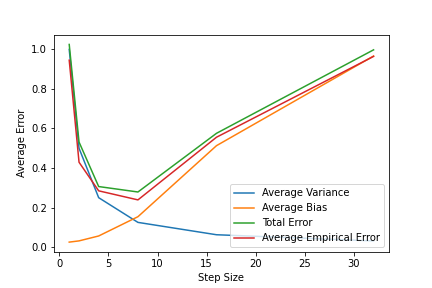
\includegraphics[width=10cm, height=7cm]{pic_1}

\subsection*{e.}

In the average bias squared expression $\frac{1}{n} \sum_{j=1}^{n/m} \sum_{i=(j-1)m+1}^{jm} (\bar{f}^{(j)} - f(x_i))^2$, we can notice that $\frac{1}{n} \sum_{j=1}^{n/m} \sum_{i=(j-1)m+1}^{jm}$ does not make the total expression much bigger or smaller. It is only doing the summation and then do the average. I will just ignore it for a moment. 

From the question, we know that:
\[ min_{i=(j-1)m+1, \dots ,jm} f(x_i) \le \bar{f}_{(j)} \le max_{i=(j-1)m+1, \dots ,jm} f(x_i) \]
Based on the L-Lipschitz rule, we got:

\[|\bar{f}_{(j)} - f(x_i)|  \le  | max_{i=(j-1)m+1, \dots ,jm} f(x_i) - min_{i=(j-1)m+1, \dots ,jm} f(x_i) |\]
\[ |\bar{f}_{(j)} - f(x_i)|  \le \frac{L}{n}|  max_{i=(j-1)m+1} - min_{i=(j-1)m+1} |\]
\[ |\bar{f}_{(j)} - f(x_i)|  \le  \frac{L}{n} |m| \]
Recall that each interval has m elements
\begin{subequations}
\begin{align*}
(\bar{f}_{(j)} - f(x_i))^2 & \le (\frac{L}{n} |m|)^2 \\
& \le \frac{L^2m^2}{n^2}
\end{align*}
\end{subequations}
As for the total error, and recall $\sigma^2 = 1$, \newline
\[ (\bar{f}_{(j)} - f(x_i))^2 + \frac{\sigma^2}{m} \le \frac{L^2(m)^2}{n^2} + \frac{1}{m} \]

Minimizing the total error with respect to m.
\[\frac{dO}{dm} = \frac{2L^2m}{n^2} - m^{-2}\]
\[0 = \frac{2L^2m}{n^2} - m^{-2}\]
\[m = (\frac{n^2}{2L^2})^{\frac{1}{3}}\]

From above, we know that m can not be 0, can not be negative. And it is really intuitive that when m increases, the bias term decrease, and variance increase. It make sense that it need to find a balance point according to the data size. Also we can see that there is a positive relationship between m and n, and there is a negative relationship between n and L.


For this particular scenario, n is 256, and we can see the lowest valley is when m is 8.
\[8 = (\frac{256^2}{2L^2})^{\frac{1}{3}}\]
\[L = 8\]






\section*{B.2}
\subsection*{a.}


\begin{minted}[mathescape,linenos,obeytabs=true,tabsize=2]{python}

import numpy as np
import matplotlib.pyplot as plt
import mnist

mndata = mnist.MNIST('./python-mnist/data/')
X_train, labels_train = map(np.array, mndata.load_training())
X_test, labels_test = map(np.array, mndata.load_testing())
X_train = X_train/255.0
X_test = X_test/255.0
# This function trains the model the return the weights
def train(X, Y):
	lambda_ = 0.0001
	n, d = np.shape(X)
	W = np.linalg.solve(X.T @ X + lambda_ * np.identity(d), X.T @ Y)
	return W

# This function do the prediction
def predict(W,X):
	return (X @ W).argmax(axis = 1)

# This function apply the transformation to data
def h1(X_train, X_test, p):
	n, d = X_train.shape
	sigma = np.sqrt(0.1)
	G = np.random.normal(0, sigma, p * d).reshape(p, d)
	b = np.random.uniform(0, 2 * np.pi, p).reshape(p, 1)
	h_train = np.cos(np.dot(X_train, G.T) + b.T)
	h_test = np.cos(np.dot(X_test, G.T) + b.T)
	
	return h_train, h_test, G, b

n, d = X_train.shape
training_error_all = []
validing_error_all = []
W_list = []
Gb_list = []
train_index = np.random.choice(np.arange(n), int(X_train.shape[0] * 0.8), replace=False)
valid_index = np.setdiff1d(np.arange(n), train_index)
# loop from p=500 to p=6000, step=500
for p in list(range(500, 6001, 500)):
	h_train, h_test, G, b = h1(X_train[train_index, :], X_train[valid_index, :], p)
	# h = h1(X_train, p)
	# Train test split with 80%-20%    
	Gb_list.append((G,b))
	train_data = h_train
	valid_data = h_test
	y_train = np.eye(10)[labels_train[train_index]]
	
	# Compute weights
	W_hat = train(train_data, y_train)
	W_list.append(W_hat)
	# Compute train predicted
	predict_train = predict(W_hat, train_data)
	predict_train = labels_train[train_index] - predict_train
	train_error_single = np.count_nonzero(predict_train) / len(predict_train) #train_size
	training_error_all.append(train_error_single)
	# Compute test predicted
	predicted_test = predict(W_hat, valid_data)
	predicted_test = labels_train[valid_index] - predicted_test
	valid_error_single = np.count_nonzero(predicted_test) / len(predicted_test)
	validing_error_all.append(valid_error_single)
	
	print("p: ", p,", train_err: ", train_error_single, ", test_err: ", valid_error_single)

x_index = list(range(500, 6001, 500))
plt.plot(x_index, training_error_all, label="Training Error")
plt.scatter(x_index, training_error_all)
plt.plot(x_index, validing_error_all, label="Testing Error")
plt.scatter(x_index, validing_error_all)
plt.xlabel("P")
plt.ylabel("Prediction Error Rate")
plt.legend()
\end{minted}

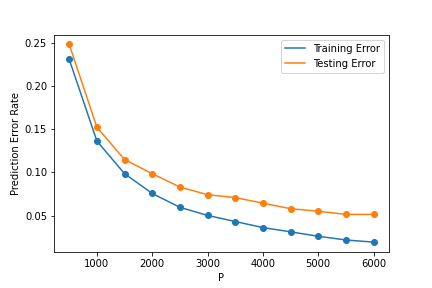
\includegraphics[width=10cm, height=7cm]{pic_2}





\subsection*{b.}

From the question, we could have:
\[ \frac{1}{m} \sum_{i=1}^{m} x_i -  \sqrt{\frac{\log(\frac{2}{\delta})}{2m}} \le  \mu \le \frac{1}{m} \sum_{i=1}^{m} x_i +  \sqrt{\frac{\log(\frac{2}{\delta})}{2m}}  \]

And $ \frac{1}{m} \sum_{i=1}^{m} x_i$ is basically the mean test error.

\begin{minted}[mathescape,linenos,obeytabs=true,tabsize=2]{python}
n, d = X_train.shape
p = 6000
dt = 0.05
sigma = np.sqrt(0.1)

h_train, h_test, G, b = h1(X_train, X_test, p)
y_train = np.eye(10)[labels_train]

# Compute weights
W_hat = train(h_train, y_train)
# Compute test predicted
predicted_test = predict(W_hat, h_test)
valid_error_single = 1 - (sum(labels_test == predicted_test) / len(labels_test))

H = np.sqrt(np.log(2/dt)/(2*len(labels_test)))
print(f'The test_error is {valid_error_single}')
print(f'Confidence Interval:[{valid_error_single - H} : {valid_error_single + H}]')
# The test_error is 0.04600000000000004
# Confidence Interval:[0.03241898484259385 : 0.059581015157406235]
\end{minted}












\end{document}